\section{Experiments}
\label{sec:results}
\label{sec:main-results}

\begin{figure}[t]
\centering

\includegraphics[width=\columnwidth]{f2_regime_scatter_v2}
\caption{SICA $\Delta$ (pp) vs.\ SC baseline. Color: model family; shape: dataset (\scalebox{0.7}{$\blacksquare$}\,PW, \scalebox{0.7}{$\blacktriangle$}\,FOLIO, \scalebox{0.7}{$\bullet$}\,LogiQA). Circled: significant ($p < .05$). Grey band: $\pm 2$\,pp equivalence zone. Three regimes emerge: Type~C (error amplification), intermediate, and Type~A (confirmation bias).}
\label{fig:regime-scatter}
\end{figure}

\subsection{Experimental Setup}
\label{sec:exp-setup}

\looseness=-1
\paragraph{Models.} Qwen2.5-14B-Instruct, Qwen2.5-7B-Instruct, Qwen3-14B (non-thinking mode)~\citep{yang2024qwen25}, Mistral-7B-Instruct-v0.3~\citep{jiang2023mistral}, LLaMA-3.1-8B-Instruct~\citep{dubey2024llama3}, and QwQ-32B~\citep{qwen2024qwq} (7B--32B). We also evaluate the universality of symbolic confirmation bias on six additional models: gpt-4o uses self-extraction via API; four frontier models (gpt-4.1, gpt-5.5, o3, Gemini-2.5-Pro) use cross-model extraction where Mistral-7B extracts constraints from target traces; DeepSeek-R1-Distill-Qwen-8B likewise uses Mistral-7B cross-extraction (Table~\ref{tab:frontier-scb}).

\paragraph{Datasets.} FOLIO~\citep{han2022folio} ($n{=}204$, gold logical annotations), ProofWriter depth-5~\citep{tafjord2021proofwriter} ($n{=}600$), LogiQA~\citep{liu2020logiqa} ($n{=}200$), StrategyQA~\citep{geva2021strategyqa} ($n{=}200$). GSM8K ($n{=}30$) and AIME 2024 ($n{=}22$) probe the degenerate regime ($C_0 < 5\%$).

\paragraph{Parameters.} $K{=}12$ traces at $T{=}0.7$, extraction at $T_{\text{ext}}{=}0.3$, $\alpha{=}0.5$, Z3 timeout 10s (K-sensitivity and extraction-temperature analysis in Appendix~\ref{app:sensitivity}). McNemar exact test ($\alpha{=}0.05$); 95\% bootstrap CIs ($10{,}000$ resamples; Appendix~\ref{app:bootstrap}) for $n \geq 200$. SICA incurs $4.5{\times}$ SC wall-clock; extraction accounts for 76\% of overhead.

\subsection{Main Results}

\looseness=-1 Table~\ref{tab:main_results} reports accuracy across all non-degenerate self-extraction conditions sorted by SC baseline. Two confirmatory conditions show significant degradation after BH correction for false discovery rate ($m{=}6$; multi-seed aggregates and extensions are exploratory): Mistral-7B on ProofWriter ($-2.83$\,pp, raw $p = 0.014$, adj.\ $p = 0.042$) and Qwen2.5-14B on ProofWriter ($-2.50$\,pp, raw $p = 0.011$, adj.\ $p = 0.042$). No condition shows a significant positive effect. An aggregate sign test yields 8 positive and 7 negative $\Delta$ values ($p = 1.00$, two-sided). When SICA and SC disagree, SC selects the correct answer $2.6\times$ more often (139 vs.\ 53 across conditions); constraint-based reweighting thus introduces noise rather than corrective signal (representative cases in Appendix~\ref{app:case-studies}; Appendix~\ref{app:subpopulation}).

\begin{figure}[t]
\centering
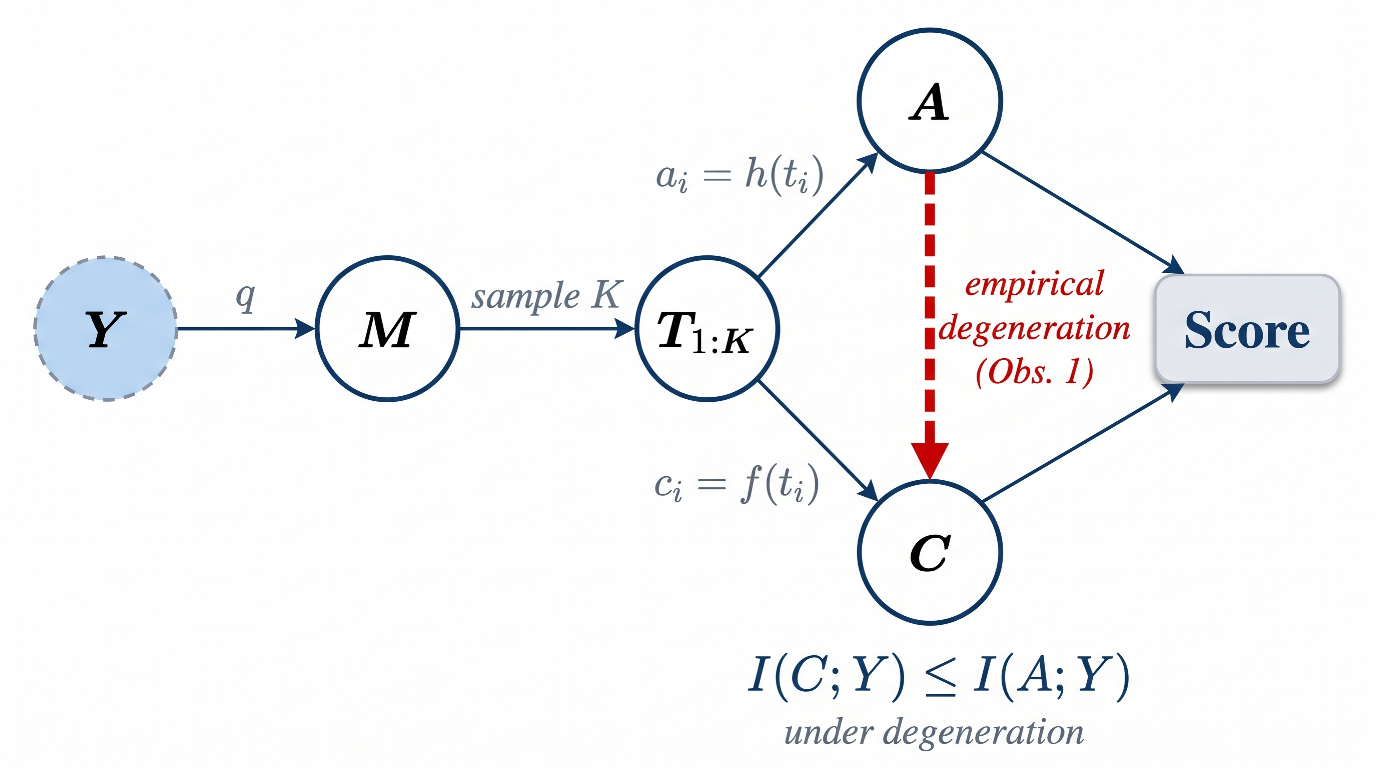
\includegraphics[width=\columnwidth]{figures/fig3_causal_dag_v12.pdf}
\caption{Causal DAG of the self-extraction pipeline. Traces $T$ produce both answers $A$ and constraints $C$; under degeneration (Observation~1), $C$ is determined by $A$ (dashed arrow), yielding $I(C;Y) \leq I(A;Y)$.}
\label{fig:causal-dag}
\end{figure}

\looseness=-1 Figure~\ref{fig:regime-scatter} reveals regime structure across SC baselines. Three regimes emerge: Type~C (SC $\leq 40\%$), where low accuracy causes error amplification; an intermediate band (50--60\%), containing the only positive trends; and Type~A (SC $\geq 60\%$), where symbolic confirmation bias dominates. Fleiss' $\kappa$ ranges from 0.19 to 0.82, yielding $K_{\text{eff}} = 1.20\text{--}3.94$ at $K = 12$ (Table~\ref{tab:independence}; Appendix~\ref{app:cross-model-kappa}). Seed-level noise is substantial: across three Mistral-7B seeds, $\Delta$ ranges from $+2.94$ to $-2.45$\,pp despite $\kappa \in [0.45, 0.46]$. We trace the mechanism in \S\ref{sec:analysis}.

\looseness=-1 We use TOST equivalence tests \citep{lakens2017equivalence} with margin $\pm 2$\,pp, justified on four grounds: (1)~on FOLIO ($n{=}204$), $\pm$2\,pp corresponds to ${\sim}$4 problems, near single-item influence; (2)~multi-seed SC variability $\sigma_{\text{SC}} = 1.67$--$2.51$\,pp on FOLIO, with $\sigma_\Delta$ up to 2.70\,pp (Table~\ref{tab:multi-seed}), placing $\pm$2\,pp within natural noise; (3)~the observed $|\Delta|$ median across 11 conditions is 1.47\,pp, so $\pm$2\,pp captures the central tendency; (4)~sensitivity analysis confirms $\pm$2\,pp as the narrowest discriminating window ($\pm$1\,pp: zero conditions pass; $\pm$3\,pp: all pass; Appendix~\ref{app:tost}). Four of 11 conditions pass TOST equivalence (minimum detectable effect (MDE) $\leq 2$\,pp); the remaining seven are underpowered (MDE $4.6$--$4.8$\,pp) but provide consistent directional evidence ($|\Delta| \leq 4.41$\,pp, none significant; Appendix~\ref{app:power}). Multi-seed replication: mean $\Delta = +0.16 \pm 2.70$\,pp across three Mistral-7B seeds (Table~\ref{tab:multi-seed}); four Qwen2.5-14B seeds yield $\Delta \in [0.00, -2.01]$\,pp; four Qwen3-14B seeds yield $\Delta = +0.92 \pm 1.14$\,pp (n.s.; Appendix~\ref{app:single-trace}). Oracle controls confirm the MAX-SAT mechanism is sound ($+29.90$/$+13.73$\,pp FOLIO, $+17.17$\,pp ProofWriter; $p < 0.001$), yet self-extraction captures only ${\sim}12\%$ of this ceiling (Appendix~\ref{app:oracle}; Appendix~\ref{app:pw-oracle-subtype}).

